%-----------------------------------
\newcommand{\meta}[2]{
	\begin{frame}
		\frametitle{#1}
		\centering
		{\fontsize{5cm}{1em}\selectfont \textbf{#2}}
	\end{frame}
}
%-----------------------------------


\section{Metacaracteres}
\frame{\tableofcontents[currentsection]}

\subsection{Caracteres e Metacaracteres}

\begin{frame}
	\frametitle{Você sabe o que são os metacaracteres?}
	
	\begin{itemize}
		\item Se você não conhecia essas belezinhas de \textit{expressões regulares} você só utilizou caracteres literais durante toda sua vida;

		\item Metacaracteres, você, você metacaracteres;

		\item Como isso vai fazer diferença na minha vida?

		\item Diferença dos robozinhos.		
	\end{itemize}
\end{frame}

\begin{frame}
	\begin{figure}
		\centering
			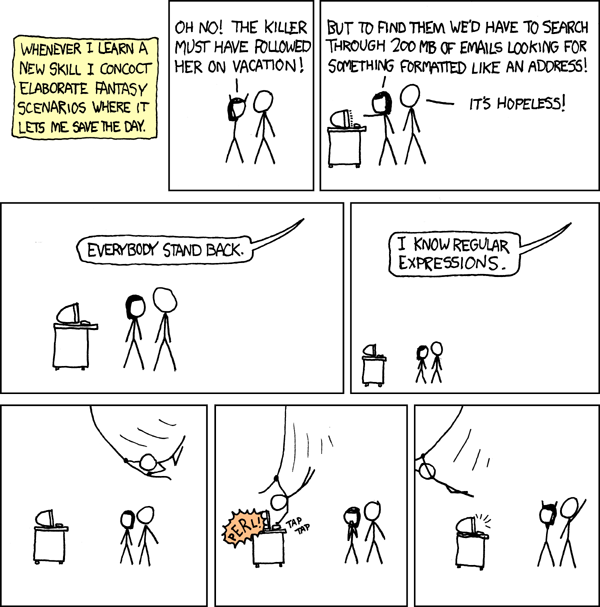
\includegraphics[height=0.8\textheight]{imagens/re/regular_expressions.png}
		\caption{Expressões Regulares salvando o dia}
	\end{figure}

\end{frame}

\begin{frame}
	\frametitle{Tipos}
	\Large{\azul{Representante}, \azul{Quantificador} e \azul{Âncora}}
\end{frame}

\subsection{Observações}
\meta{Grupo}{(...)}
\meta{Escape}{\textbackslash n}

\subsection{Tipo Representante}

%------------------------------------------------
\meta{Ponto}{.}

\begin{frame}
	\frametitle{O ponto}
	\begin{itemize}
		\item \Large{O ponto casa com \azul{TUDO}.}
		\item i.e., o ponto casa com qualquer caractere!
		\item \azul{Pergunta}: o ponto casa com um ponto?
	\end{itemize}
\end{frame}

\begin{frame}
	\begin{figure}
		\centering
		
\includegraphics[height=0.8\textheight]{./imagens/re/sad_joker.jpeg}
		\caption{O ponto é o coringa solitário.}
	\end{figure}
\end{frame}

\begin{frame}
	\frametitle{Casamento do ponto}
	\begin{center}
		\begin{tabular}{ c | c }
		\textbf{Expressão}	& \textbf{Casa com...}		\\ \hline
		n.o			& nao, não, n4o, noo...  	\\ \hline
		.u			& au, bu, du...		 	\\ \hline
		12.45			& 12:45, 12 45, 12.45... 	\\ \hline
		\end{tabular}
	\end{center}

\end{frame}

%------------------------------------------------
\meta{Lista}{[...]}

\begin{frame}
	\frametitle{A lista}
	\begin{itemize}
		\item \Large{A lista casa com \azul{TODOS} os caracteres dentro dela.}
		\item \textbf{Exemplos}: [abc], [123], [letras]...
		\item \large{\bf Dentro da lista todo mundo é LITERAL.}
		\begin{itemize}
			\item O ponto dentro da lista é literal;
		\end{itemize}
	\end{itemize}
\end{frame}

\begin{frame}
	\frametitle{Mentiroso!}
	\begin{itemize}
		\item Lembra que eu falei que todo mundo dentro lista era literal? Então... \Large{\bf EU MENTI \vermelho{MUAHAHAHA}}.
	\end{itemize}
\end{frame}

\begin{frame}
	\frametitle{Mentiroso (nem tanto, vai)!}
	\begin{itemize}
		\item Lembra que eu falei que todo mundo dentro lista era literal? Então...
		\begin{itemize}
			\item Todo caractere que se acha fora da lista, lá dentro não serve pra nada ou tem outro significado;
			\item É como se ela tivesse um mundinho dentro dela, só dela, onde ela dita as regras.
		\end{itemize}
	\end{itemize}
\end{frame}
%------------------------------------------------
\meta{Lista Negada}{[\textasciicircum...]}

\begin{frame}
	\frametitle{A lista negada}
	\begin{itemize}
		\item \Large{A \azul{lista negada} casa com \azul{TODOS} os caracteres que \textbf{\vermelho{NÃO}} estão dentro dela.}
		\item Ou seja, ela não é tão seletiva quanto a lista, tampouco liberal quanto o ponto. Ela sabe com quem não quer casar;
		\item \textbf{Exemplos}: [\textasciicircum abc], [\textasciicircum 123], [\textasciicircum letras]...
	\end{itemize}
\end{frame}

%SOBRE LISTAS--------------------------------------
\begin{frame}
	\frametitle{Intervalos}
	
	\begin{itemize}
		\item Como você faria uma expressão regular para casar com dois números consecutivos?
	\end{itemize}
\end{frame}

\begin{frame}
	\frametitle{Intervalos}
	
	\begin{itemize}
		\item Como você faria uma expressão regular para casar com dois números consecutivos?
		\begin{itemize}
			\item "\textbf{[0123456789][0123456789]}"?
		\end{itemize}
	\end{itemize}
\end{frame}

\begin{frame}
	\frametitle{Intervalos}

	\begin{itemize}
		\item O traço (-) é um operador não literal dentro da lista;
		\item Ele foi criado para representar intervalos:
			\begin{itemize}
				\item \lista{0-9} é igual a \lista{0123456789};
				\item \lista{a-z} é igual a \lista{abcdefghijklmnopqrstuvwxyz};
				\item \lista{A-Z} é igual a \lista{ABCDEFGHIJKLMNOPQRSTUVWXYZ};
				\item \lista{0-9a-zA-Z}
				\item \lista{ -\textasciitilde}
			\end{itemize}
	\end{itemize}
\end{frame}

\begin{frame}
	\frametitle{Intervalos}

	\begin{itemize}
		\item O traço (-) é o único operador não literal dentro da lista;
		\item Ele foi criado para representar intervalos:
			\begin{itemize}
				\item \lista{0-9} é igual a \lista{0123456789};
				\item \lista{a-z} é igual a \lista{abcdefghijklmnopqrstuvwxyz};
				\item \lista{A-Z} é igual a \lista{ABCDEFGHIJKLMNOPQRSTUVWXYZ};
				\item \lista{0-9a-zA-Z};
				\item \lista{ -\textasciitilde}\Huge{\bf \vermelho{???}}
			\end{itemize}
	\end{itemize}
\end{frame}

\begin{frame}
	\frametitle{Exceções}
	
	\begin{itemize}
		\item \textbf{E se eu quiser colocar um traço (-) na lista?}
		\item \textbf{E se eu quiser colocar os colchetes (\lcol  e \rcol) na lista?}
		\item \textbf{E se eu quiser colocar um circunflexo na lista?}
		\item \textbf{E se...}
	\end{itemize}

\end{frame}

\begin{frame}
	\frametitle{Exceções}
	
	\begin{itemize}
		\item \textbf{E se eu quiser colocar um traço (-) na lista?}
		\begin{itemize}
			\item Devemos color o traço no começo ou no final da lista;
			\item \lista{-0-9} $\rightarrow$ Casa com 0 a 9 e traço;
			\item \lista{a-f-} $\rightarrow$ Casa com a a f e traço;
		\end{itemize}
		\item \textbf{E se eu quiser colocar os colchetes (\lcol  e \rcol) na lista?}
		\item \textbf{E se eu quiser colocar um circunflexo na lista?}
		\item \textbf{E se...}
	\end{itemize}

\end{frame}

\begin{frame}
	\frametitle{Exceções}
	
	\begin{itemize}
		\item \textbf{E se eu quiser colocar um traço (-) na lista?}
		\item \textbf{E se eu quiser colocar os colchetes (\lcol  e \rcol) na lista?}
		\begin{itemize}
			\item O "colchete abrir" podemos colocar em qualquer lugar:
			\begin{itemize}
				\item \lista{\lcol0-9};
				\item \lista{0-4\lcol*.ç};
			\end{itemize}
			\item O "colchete de fechar" deve ser o primeiro da lista;
			\begin{itemize}
				\item \lista{\rcol0-9} $\rightarrow$ Casa com 0 a 9 ou com \rcol.
				\item \lista{0-9\rcol} $\rightarrow$ Tá errado.
			\end{itemize}
		\end{itemize}
		\item \textbf{E se eu quiser colocar um circunflexo na lista?}
		\item \textbf{E se...}
	\end{itemize}

\end{frame}

\begin{frame}
	\frametitle{Exceções}
	
	\begin{itemize}
		\item \textbf{E se eu quiser colocar um traço (-) na lista?}
		\item \textbf{E se eu quiser colocar os colchetes (\lcol  e \rcol) na lista?}
		\item \textbf{E se eu quiser colocar um circunflexo na lista?}
			\begin{itemize}
				\item \lista{a-z\textasciicircum}$\rightarrow$casa com caracteres de a a z e \textasciicircum;
				\item \lista{\textasciicircum a-z}$\rightarrow$lista negada: casa com qualquer coisa que não seja de a a z.
			\end{itemize}
		\item \textbf{E se...}
	\end{itemize}

\end{frame}

\begin{frame}
	\frametitle{Exceções}
	
	\begin{itemize}
		\item \textbf{E se eu quiser colocar um traço (-) na lista?}
		\item \textbf{E se eu quiser colocar os colchetes (\lcol  e \rcol) na lista?}
		\item \textbf{E se eu quiser colocar um circunflexo na lista?}
		\item \textbf{E se...}
		\begin{itemize}
			\item Mais alguma coisa/dúvida?
		\end{itemize}
	\end{itemize}

\end{frame}

\begin{frame}
	\frametitle{Casamento das listas}
	\begin{center}
	\begin{tabular}{ c | c }
		\textbf{Expressão} & \textbf{Casa com...} \\ \hline
		n[aãAÃ]o	&	nao, não, nAo, nÃo \\ \hline
		12[:. ]45	&	12:45, 12.45, 12 45 \\ \hline
		funcao.[ch]	&	funcao.c, funcao.h   \\ \hline
		[][-]		&	\textbf{???}		\\ \hline

	\end{tabular}
	\end{center}
\end{frame}

\begin{frame}
	\frametitle{Casamento das listas}
	\begin{center}
	\begin{tabular}{ c | c }
		\textbf{Expressão} & \textbf{Casa com...} \\ \hline
		n[aãAÃ]o	&	nao, não, nAo, nÃo \\ \hline
		12[:. ]45	&	12:45, 12.45, 12 45 \\ \hline
		funcao.[ch]	&	funcao.c, funcao.h   \\ \hline
		[][-]		&	[, ], -		\\ \hline
	\end{tabular}
	\end{center}
\end{frame}

%------------------------------------------------
\subsection{Tipo Quantificador}

%------------------------------------------------
\meta{Opcional}{?}

\begin{frame}
	\frametitle{O opcional}
	\begin{itemize}
		\item O opcional torna um caractere ou metacaractere de representação anterior em opcional;
		\item Sua \azul{cardinalidade} é 0 ou 1;
	\end{itemize}
\end{frame}

\begin{frame}
	\frametitle{O casamento do opcional}
	
	\begin{center}
	\begin{tabular}{c | c}
		\textbf{Expressão} 	& \textbf{Casa com...} \\ \hline
		fala[r!]?		& fala, falar, fala! 	\\ \hline
		pessoas?		& pessoa, pessoas 	\\ \hline
		(hiper)?mercado		& hipermercado, mercado \\ \hline
	\end{tabular}
	\end{center}
\end{frame}

%------------------------------------------------
\meta{Asterisco}{*}

\begin{frame}
	\frametitle{O asterisco}
	\begin{itemize}
		\item O asterisco é o guloso;
		\item A cardinalidade dele é 0 ou 1 até \azul{infinito}!
	\end{itemize}
\end{frame}

\begin{frame}
	\frametitle{O casamento do asterisco}
	
	\begin{center}
	\begin{tabular}{c | c}
		\textbf{Expressão} 	& \textbf{Casa com...} \\ \hline
		an*a			& , ana, annnnna, annnnnna... 	\\ \hline
		[ar]*a			& arara, a, aararrarra... 	\\ \hline
		10*			& 1, 100, 1000000000... \\ \hline
	\end{tabular}
	\end{center}
\end{frame}

\meta{Gulodice sem fim}{.*}

\begin{frame}
	\frametitle{Apresentando a gulodice infinita}

	\begin{itemize}
		\item Esses dois operadores juntos são muito úteis;
		\item Com grandes poderes vêm grandes responsabilidades;
		\item Esses operadores juntos casam com qualquer coisa, em qualquer quantidade;
	\end{itemize}
\end{frame}

\begin{frame}
	\frametitle{Máquina de estados}

	\begin{figure}
		\centering
		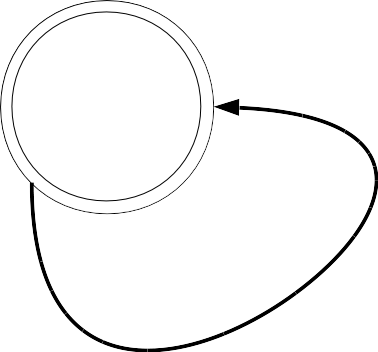
\includegraphics[height=.75\textheight]{./imagens/re/maq_estados.png}
		\caption{Máquina de estados da expressão .*}
	\end{figure}

\end{frame}

%%------------------------------------------------
\meta{Mais}{+}

\begin{frame}
	\frametitle{O mais}
	\begin{itemize}
		\item É igual ao asterisco só que não é opcional;
		\item \azul{\textbf{Tem}} que ter o caractere que está sendo quantificado;
		\item A cardinalidade do operador mais é 1 até infinito.
	\end{itemize}
\end{frame}

\begin{frame}
	\frametitle{Casamento do Mais}
	\begin{center}
	\begin{tabular}{c|c}
		\textbf{Expressão} & \textbf{Casa com...} \\ \hline
		an+a		& ana, annna, annnnnnna \\ \hline
		cobras+		& cobras, cobrasssssssss \\ \hline
		10+		& 10, 100, 100		\\ \hline
	\end{tabular}
	\end{center}
\end{frame}

%------------------------------------------------
\meta{Chaves}{ \{m,n\} }

\begin{frame}

	\frametitle{As Chaves}
	\begin{itemize}
		\item As chaves tem um comportamento que consegue simular os operadores opcional(?), asterisco(*) e mais(+);
		\item Ele pode as seguintes "caras":
		\begin{enumerate}
			\item \textbf{\{n\}}: repetir \textbf{n} vezes;
			\item \textbf{\{n,m\}}: repetir de \textbf{n} até \textbf{m};
			\item \textbf{\{n,\}}: repetir de \textbf{n} até infinito;
			\item \textbf{\{,m\}}: repetir até \textbf{m} vezes.
		\end{enumerate}
		\item \azul{Pergunta}: Como o operador consegue simular os operadores \textbf{?}, \textbf{*} e \textbf{+}?
	\end{itemize}
\end{frame}

\begin{frame}
	\frametitle{Respostas}
	\begin{itemize}
		\item \textbf{?}: \{1\}
		\item \textbf{*}: \{0,\}
		\item \textbf{+}: \{1,\}
	\end{itemize}
\end{frame}

%------------------------------------------------
\subsection{Tipo Âncora}

%------------------------------------------------
\meta{Circunflexo}{\textasciicircum}

\begin{frame}
	\frametitle{O Circunflexo}

	\begin{itemize}
		\item O circunflexo casa com o começo da linha;
		\item Não confunda com o caractere da lista!
		\item O circunflexo só tem função de âncora no começo da linha, obviamente;
		\item i.e. o caractere circunflexo (\textasciicircum) vai ser literal no meio da linha.
	\end{itemize}
\end{frame}

\begin{frame}
	\frametitle{O casamento do circunflexo}
	\begin{center}
	\begin{tabular}{c|c}
		\textbf{Expressão} & \textbf{Casa com...} \\ \hline
		\textasciicircum a & Todas  as linhas que começam com a \\ \hline
		\textasciicircum \textasciicircum & Todas as linhas que começam com \textasciicircum \\ \hline
	\end{tabular}
	\end{center}
\end{frame}

%------------------------------------------------
\meta{Cifrão}{\$}

\begin{frame}
	\frametitle{O cifrão}

	\begin{itemize}
		\item O cifrão casa com o final da linha;
		\item O cifrão é literal no meio da linha;
	\end{itemize}
\end{frame}

\begin{frame}
	\frametitle{O casamento do cifrão}

	\begin{center}
	\begin{tabular}{c|c}
		\textbf{Expressão} & \textbf{Casa com...} \\ \hline
		a\$		& Uma linha que termina com a \\ \hline
		\textasciicircum .\{40\}\$ & Uma linha com 40 caracteres \\ \hline
		\textasciicircum \$ & \textbf{???}		\\ \hline
	\end{tabular}
	\end{center}

\end{frame}

\begin{frame}
	\frametitle{O casamento do cifrão}

	\begin{center}
	\begin{tabular}{c|c}
		\textbf{Expressão} & \textbf{Casa com...} \\ \hline
		a\$		& Uma linha que termina com a \\ \hline
		\textasciicircum .\{40\}\$ & Uma linha com 40 caracteres \\ \hline
		\textasciicircum \$ & \textbf{Uma linha vazia}		\\ \hline
	\end{tabular}
	\end{center}

\end{frame}
%------------------------------------------------
\meta{Borda}{\textbackslash b}
\begin{frame}
	\frametitle{A borda}

	\begin{itemize}
		\item Casa com a borda das palavras;
		\item Definição de borda: espaço depois de letras;
	\end{itemize}
\end{frame}

\begin{frame}
	\frametitle{O casamento da borda}
	\begin{center}
	\begin{tabular}{c|c}
		\textbf{Expressão} & \textbf{Casa com...} \\ \hline
		\textbackslash bdia & dia, diafragma, bom-dia! \\ \hline
		\textbackslash bdia & dia, diafragma, bom-dia! \\ \hline
		dia\textbackslash b & dia, melodia, bom-dia! \\ \hline
		\textbackslash bdia\textbackslash b& dia, bom-dia! \\ \hline
	\end{tabular}
	\end{center}
	
\end{frame}


%------------------------------------------------
\subsection{Outros}

%------------------------------------------------
\meta{Ou}{|}

\begin{frame}
	\frametitle{O ou}
	\begin{itemize}
		\item É um operador lógico, casa com a ou b, onde a e b são expressões regulares;
		\item \textbf{Exemplo}: $a|b$;
	\end{itemize}
\end{frame}

\begin{frame}
	\frametitle{Casa com...?}
	\Huge{\bf mal(a|inha|eta)}
\end{frame}

\begin{frame}
	\frametitle{Casa com...?}
	\Huge{\bf bols(a|inha)}
\end{frame}

\begin{frame}
	\frametitle{Casa com...?}
	\Huge{\bf pern(a|inha|eta)}
\end{frame}

\begin{frame}
	\frametitle{Casa com...?}
	\Huge{\bf punh(o|inho)}
\end{frame}

%------------------------------------------------
\meta{Retrovisor}{\textbackslash 1...\textbackslash 9}

\begin{frame}
	\frametitle{O retrovisor}

	\begin{itemize}
		\item O retrovisor "olha" para os grupos "(...)";
		\item O vão de \textbackslash 1 a \textbackslash 9;
	\end{itemize}
\end{frame}

\begin{frame}
	\frametitle{O casamento da borda}
	\begin{center}
	\begin{tabular}{c|c}
		\textbf{Expressão} & \textbf{Casa com...} \\ \hline
		(quero)-\textbackslash 1	& quero-quero \\ \hline
		([A-Za-z]+)-\textbackslash 1  & qualquerpalavra-qualquerpalavra \\ \hline
	\end{tabular}
	\end{center}

\end{frame}
%------------------------------------------------
